\chapter{Contraction Hierarchies, Hierarchical Hub Labelings}\label{chapter:ch}

Mit dem Aufkommen von Online-Kartendiensten stieg der Bedarf an effizienten Algorithmen zur Berechnung von kürzesten Pfaden in großen Netzwerken stark an.
cite{geisberger2008contraction} stellte hierfür \emph{Contraction Hierarchies} vor, eine Methode, die ein ähnliches Konzept wie die in \autoref{graphs:strassengraphen} vorgestellte Idee der Wichtigkeit von Kanten nutzt und auf Straßengraphen einen Speedup um mehrere Größenordnungen ermöglicht.
Darauf aufbauend stellte \cite{abraham2011hub} eine logische Weiterentwicklung vor, welche einen mit \emph{Contraction Hierarchies} bearbeiteten Graph als Eingabe erwartet.
Sie ermöglicht auf Straßengraphen noch einmal einen Speedup um einige Größenordnungen.
Im Folgenden werden die Grundlagen dieser Ansätze erläutert und ihre Anwendung auf Sichtbarkeitsgraphen diskutiert.

\section{Contraction Hierarchies}

Die Grundidee der Contraction Hierarchies ist es, aus einem Graph zwei Graphen zu erzeugen, in denen die Suche nur einen kleinen Teil aller Knoten findet, es jedoch deutlich günstiger in ihnen zu suchen.
Durch die spezielle Konstruktion dieser Graphen ist garantiert, dass die Suche vom Startknoten aus in dem einen und die Suche vom Zielknoten aus in dem anderen Graphen einen Knoten findet, der auf dem kürzesten Pfad zwischen dem Startknoten und dem Zielknoten liegt.
Der kürzeste Pfad kann dann, wie bei einer bidirektionalen Dijkstra-Suche, aus den Teilsuchen erstellt werden.

\subsection{Knoten Kontraktion}

Der Name Contraction Hierarchies leitet sich aus dem Konzept der Knoten Kontraktion (Contraction) ab.

\begin{definition}[Knoten Kontraktion]
    Sei $G = (V, E)$ ein Graph. Sei $v \in V$ der zu kontraktierende Knoten. Die Kontraktion von $v$ erfolgt durch:

    \begin{enumerate}
        \item\label{ch:contraction:when_shortcut}
        Für jeden Vorgänger $u \in V$ und jeden Nachfolger $w \in V$ von $v$ wird, wenn $v$ auf dem einzigen kürzesten Pfad zwischen $u$ und $w$ liegt, eine Abkürzungskante (Shortcut) $(u, w, w_{uw})$ zu $E$ hinzugefügt.

        \item
              Alle Kanten von und zu $v$ entfernt werden.
    \end{enumerate}
\end{definition}

Nach der Kontraktion $v$ ist also isoliert.
Um die Abkürzungen zu erzeugen, kann von jedem Vorgänger eine modifizierte Dijkstra-Suche zu allen Nachfolgern ausgeführt werden, bei der keine Kanten von und zu $v$ begangen werden.
Ist die Länge der potenziellen Abkürzung kürzer als die des in der modifizierten Dijkstra-Suche gefundenen Pfades, so liegt $v$ auf dem einzigen kürzesten Pfad zwischen $u$ und $w$.
Diese Kontraktion bewahrt die kürzesten Pfaddistanzen zwischen den verbleibenden Knoten..

Betrachten wir dies wieder am Beispielgraph.
Sei $i$ der zu kontraktierende Knoten, die Nachbarn sind $a$, $b$, $j$ und $h$.
Die kürzesten $a-b$, $b-j$, $h-j$ und $a-h$ Pfade führen nicht durch $i$.
Der kürzeste $a-j$ Pfad führt jedoch über $i$.
Daher wird eine Kante zwischen $a$ und $j$ eingefügt.
\autoref{graphs:fig:example_contraction} zeigt den Graphen nach der Kontraktion.

\begin{figure}[ht]
    \centering
    \begin{subfigure}[b]{0.49\textwidth}
        \centering
        \resizebox{\textwidth}{!}{% <------ Don't forget this %
            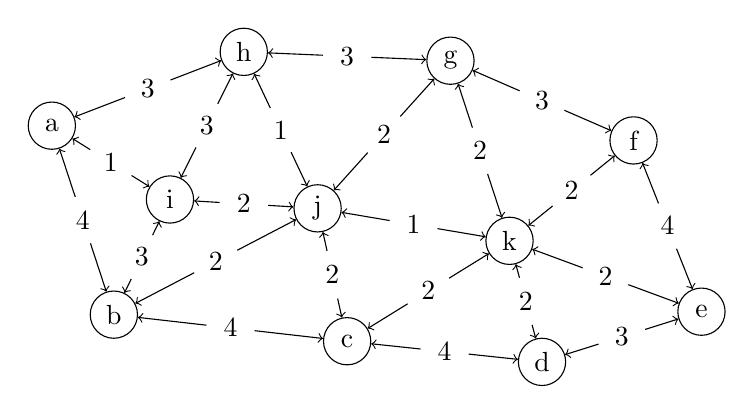
\begin{tikzpicture}[scale=0.750]
                \node[circle, draw, minimum size=0.6cm, inner sep=0pt] at (0.5* 0.0, 0.5* 8.5)  (a)    {a};
                \node[circle, draw, minimum size=0.6cm, inner sep=0pt] at (0.5* 2.1, 0.5* 2.1)  (b)    {b};
                \node[circle, draw, minimum size=0.6cm, inner sep=0pt] at (0.5* 10.0, 0.5* 1.2)  (c)    {c};
                \node[circle, draw, minimum size=0.6cm, inner sep=0pt] at (0.5* 16.6, 0.5* 0.5)  (d)    {d};
                \node[circle, draw, minimum size=0.6cm, inner sep=0pt] at (0.5* 22.0, 0.5* 2.2)  (e)    {e};
                \node[circle, draw, minimum size=0.6cm, inner sep=0pt] at (0.5* 19.7, 0.5* 8.0)  (f)    {f};
                \node[circle, draw, minimum size=0.6cm, inner sep=0pt] at (0.5* 13.5, 0.5* 10.7)  (g)    {g};
                \node[circle, draw, minimum size=0.6cm, inner sep=0pt] at (0.5* 6.5, 0.5* 11.0)  (h)    {h};
                \node[circle, draw, minimum size=0.6cm, inner sep=0pt] at (0.5* 4.0, 0.5* 6.0)  (i)    {i};
                \node[circle, draw, minimum size=0.6cm, inner sep=0pt] at (0.5* 9.0, 0.5* 5.7)  (j)    {j};
                \node[circle, draw, minimum size=0.6cm, inner sep=0pt] at (0.5* 15.5, 0.5* 4.6)  (k)    {k};


                \draw[<->]  (a) edge node[circle, fill=white] {4} (b);
                \draw[<->]  (a) edge node[circle, fill=white] {3} (h);
                \draw[<->]  (a) edge node[circle, fill=white] {1} (i);

                \draw[<->]  (b) edge node[circle, fill=white] {4} (c);
                \draw[<->]  (b) edge node[circle, fill=white] {3} (i);
                \draw[<->]  (b) edge node[circle, fill=white] {2} (j);

                \draw[<->]  (c) edge node[circle, fill=white] {4} (d);
                \draw[<->]  (c) edge node[circle, fill=white] {2} (j);
                \draw[<->]  (c) edge node[circle, fill=white] {2} (k);

                \draw[<->]  (d) edge node[circle, fill=white] {3} (e);
                \draw[<->]  (d) edge node[circle, fill=white] {2} (k);

                \draw[<->]  (e) edge node[circle, fill=white] {4} (f);
                \draw[<->]  (e) edge node[circle, fill=white] {2} (k);

                \draw[<->]  (f) edge node[circle, fill=white] {3} (g);
                \draw[<->]  (f) edge node[circle, fill=white] {2} (k);

                \draw[<->]  (g) edge node[circle, fill=white] {3} (h);
                \draw[<->]  (g) edge node[circle, fill=white] {2} (j);
                \draw[<->]  (g) edge node[circle, fill=white] {2} (k);

                \draw[<->]  (h) edge node[circle, fill=white] {3} (i);
                \draw[<->]  (h) edge node[circle, fill=white] {1} (j);

                \draw[<->]  (i) edge node[circle, fill=white] {2} (j);

                \draw[<->]  (j) edge node[circle, fill=white] {1} (k);
            \end{tikzpicture}
        }
        \caption{Vor der Kontraktion}
    \end{subfigure}
    \hfill
    \begin{subfigure}[b]{0.49\textwidth}
        \centering
        \resizebox{\textwidth}{!}{% <------ Don't forget this %
            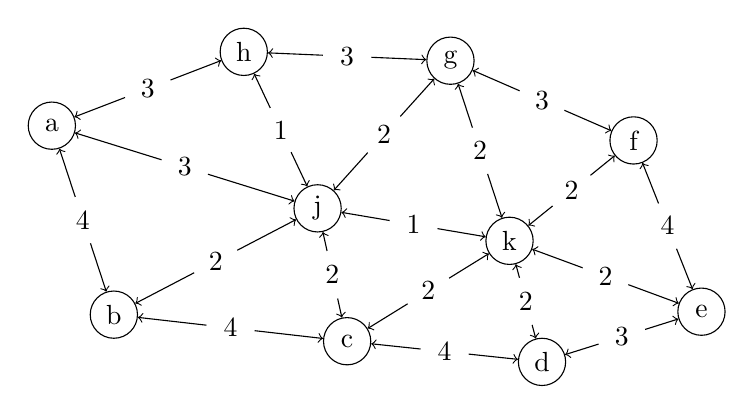
\begin{tikzpicture}[scale=0.750]
                % Nodes
                \node[circle, draw, minimum size=0.6cm, inner sep=0pt] at (0.5* 0.0, 0.5* 8.5)  (a)    {a};
                \node[circle, draw, minimum size=0.6cm, inner sep=0pt] at (0.5* 2.1, 0.5* 2.1)  (b)    {b};
                \node[circle, draw, minimum size=0.6cm, inner sep=0pt] at (0.5* 10.0, 0.5* 1.2)  (c)    {c};
                \node[circle, draw, minimum size=0.6cm, inner sep=0pt] at (0.5* 16.6, 0.5* 0.5)  (d)    {d};
                \node[circle, draw, minimum size=0.6cm, inner sep=0pt] at (0.5* 22.0, 0.5* 2.2)  (e)    {e};
                \node[circle, draw, minimum size=0.6cm, inner sep=0pt] at (0.5* 19.7, 0.5* 8.0)  (f)    {f};
                \node[circle, draw, minimum size=0.6cm, inner sep=0pt] at (0.5* 13.5, 0.5* 10.7)  (g)    {g};
                \node[circle, draw, minimum size=0.6cm, inner sep=0pt] at (0.5* 6.5, 0.5* 11.0)  (h)    {h};
                % \node[circle, draw, minimum size=0.6cm, inner sep=0pt] at (0.5* 4.0, 0.5* 6.0)  (i)    {i};
                \node[circle, draw, minimum size=0.6cm, inner sep=0pt] at (0.5* 9.0, 0.5* 5.7)  (j)    {j};
                \node[circle, draw, minimum size=0.6cm, inner sep=0pt] at (0.5* 15.5, 0.5* 4.6)  (k)    {k};


                \draw[<->]  (a) edge node[circle, fill=white] {4} (b);
                \draw[<->]  (a) edge node[circle, fill=white] {3} (h);
                \draw[<->]  (a) edge node[circle, fill=white] {3} (j);

                \draw[<->]  (b) edge node[circle, fill=white] {4} (c);
                \draw[<->]  (b) edge node[circle, fill=white] {2} (j);

                \draw[<->]  (c) edge node[circle, fill=white] {4} (d);
                \draw[<->]  (c) edge node[circle, fill=white] {2} (j);
                \draw[<->]  (c) edge node[circle, fill=white] {2} (k);

                \draw[<->]  (d) edge node[circle, fill=white] {3} (e);
                \draw[<->]  (d) edge node[circle, fill=white] {2} (k);

                \draw[<->]  (e) edge node[circle, fill=white] {4} (f);
                \draw[<->]  (e) edge node[circle, fill=white] {2} (k);

                \draw[<->]  (f) edge node[circle, fill=white] {3} (g);
                \draw[<->]  (f) edge node[circle, fill=white] {2} (k);

                \draw[<->]  (g) edge node[circle, fill=white] {3} (h);
                \draw[<->]  (g) edge node[circle, fill=white] {2} (j);
                \draw[<->]  (g) edge node[circle, fill=white] {2} (k);

                \draw[<->]  (h) edge node[circle, fill=white] {1} (j);

                \draw[<->]  (j) edge node[circle, fill=white] {1} (k);
            \end{tikzpicture}
        }
        \caption{Nach der Kontraktion}
    \end{subfigure}
    \caption{Kontraktion von $i$}
    \label{graphs:fig:example_contraction}
\end{figure}

Häufig wird die Kontraktionsbedingung abgeschwächt; es wird eine Kante eingefügt, wenn der Knoten auf \emph{einem} kürzesten Pfad liegt.
Dazu kann eine normale Dijkstra-Suche verwendet werden, bei der nur geprüft wird, ob der Knoten auf \emph{einem} kürzesten Pfad liegt.
Weiter kann die Anzahl der Hops der Suche begrenzt werden.
Dadurch können jedoch auch unnötige Kanten eingefügt werden, die nicht unbedingt für die Erhaltung der kürzesten Pfade erforderlich sind.

\subsection{Graphen Kontraktion}

Um die für die Beantwortung von Queries benötigte Datenstruktur, den \emph{Contracted Graph}, zu erstellen, müssen alle Knoten eines Graphens kontraktiert werden, wobei die Kanten, die in jedem Schritt entfernt werden, gesammelt werden.
Hierbei hat die Reihenfolge, in der dies geschieht einen großen Einfluss auf Perfomanz der nachfolgenden Kontraktionen und dem mit der Methode erzielte Speedup.
Die Reihenfolge der Kontraktion wird hierbei durch eine \emph{vertex-to-level}-Funktion angegeben, die bijektiv ist und definiert als ${vtl} \colon V \to L$ mit $L \subset \mathbb{N}$, $\abs{L} = \abs{V}$ und $\max(L) = \abs{V}$.
Der Knoten mit dem niedrigsten \emph{Level} wird dabei zuerst kontraktiert.
Ihre Umkehrfunktion wird \emph{level-to-vertex}-Funktion genannt.

\begin{definition}[Contrated Graph]
    Sei $G = (V, E)$ und $E'$ die durch die vollständige Kontraktion von $G$ erhalten Kanten mit der dazugehörigen vertex-to-level Funktion ${vtl}$.

    Ein Contracted Graph ist dann ein Tupel $C = (G_u, G_d)$. Der \emph{Upward Graph} ist dabei $G_u = (V, E_u)$ mit $E_u = \{ (t, h) \mid (t, h) \in E' \colon {vtl}(h) > {vtl}(t) \}$, der \emph{Downward Graph} ist $G_d = (V, E_d)$ mit $E_d = \{ (t, h)^T = (h, t) \mid (t, h) \in E' \colon {vtl}(h) < {vtl}(t) \}$.
\end{definition}

Der Name des Upward Graphen ergibt sich daher, dass die Suche in einem Upward Graph auf das Level bezogen nur \emph{aufwärts} geht.
In \cite{geisberger2008contraction} transponieren die Autoren die Kanten des Downard Graphens nicht, daher geht ihre Vorwärtssuche \emph{abwärts}.
Die Transposition der Kanten ist hierbei nur ein Trick, damit leichter argumentiert werden kann.

Der entstandene Graph ist azyklisch, da er nur Kanten enthält, deren Kopf ein größeres Level als ihr Fuß hat.
Die Anzahl der in einer Breitensuche gefunden Knoten ist geringer, als im Ursprungsgraph.
Diese Eigenschaften sorgen dafür, dass eine Suche in einem Upward Graph kostengünstiger sein kann.
Die in einem Upward Graph gefundenen kürzesten Pfade bilden eine untere Schranke für die tatsächlichen kürzesten Pfade; sie können jedoch auch länger sein als in $G$.

\autoref{graphs:fig:counterexample_uptimal_upward} zeigt ein Gegenbeispiel hierzu.
Die Knoten wurden in der Reihenfolge $c$, $d$, $a$, $b$ kontraktiert, wodurch der dazugehörige Upward Graph ensteht.
Der optimale $c-a$-Pfad in $G$ hat die Distanz zwei, in $G_u$ hat er jedoch die Distanz drei.

\begin{figure}[ht]
    \centering
    \begin{subfigure}[b]{0.49\textwidth}
        \centering
        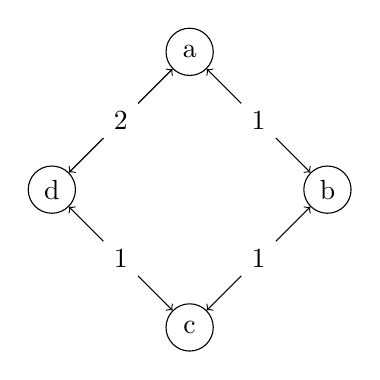
\begin{tikzpicture}
            \node[circle, draw, minimum size=0.6cm, inner sep=0pt] at (1.75*1.0, 1.75*2.0)  (a)    {a};
            \node[circle, draw, minimum size=0.6cm, inner sep=0pt] at (1.75*2.0, 1.75*1.0)  (b)    {b};
            \node[circle, draw, minimum size=0.6cm, inner sep=0pt] at (1.75*1.0, 1.75*0.0)  (c)    {c};
            \node[circle, draw, minimum size=0.6cm, inner sep=0pt] at (1.75*0.0, 1.75*1.0)  (d)    {d};

            \draw[<->]  (a) edge node[circle, fill=white] {1} (b);
            \draw[<->]  (b) edge node[circle, fill=white] {1} (c);
            \draw[<->]  (c) edge node[circle, fill=white] {1} (d);
            \draw[<->]  (d) edge node[circle, fill=white] {2} (a);
        \end{tikzpicture}
        \caption{Graph $G$}
    \end{subfigure}
    \hfill
    \begin{subfigure}[b]{0.49\textwidth}
        \centering
        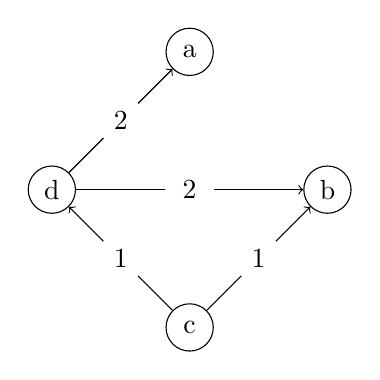
\begin{tikzpicture}
            \node[circle, draw, minimum size=0.6cm, inner sep=0pt] at (1.75*1.0, 1.75*2.0)  (a)    {a};
            \node[circle, draw, minimum size=0.6cm, inner sep=0pt] at (1.75*2.0, 1.75*1.0)  (b)    {b};
            \node[circle, draw, minimum size=0.6cm, inner sep=0pt] at (1.75*1.0, 1.75*0.0)  (c)    {c};
            \node[circle, draw, minimum size=0.6cm, inner sep=0pt] at (1.75*0.0, 1.75*1.0)  (d)    {d};

            \draw[->]  (c) edge node[circle, fill=white] {1} (b);
            \draw[->]  (c) edge node[circle, fill=white] {1} (d);
            \draw[->]  (d) edge node[circle, fill=white] {2} (b);
            \draw[->]  (d) edge node[circle, fill=white] {2} (a);
        \end{tikzpicture}
        \caption{Upward Graph $G_u$ zu $G$}
    \end{subfigure}
    \caption{Gegenbeispiel optimale Kosten im $G_u$}
    \label{graphs:fig:counterexample_uptimal_upward}
\end{figure}

\subsection{Query}

Die Suche eines kürzesten Pfades von $a$ nach $e$ auf dem Beispielgraph gestaltet sich nun wie folgt:
Auf $G_u$ wird eine Dijkstra Suche von $a$ und auf $G_d$ eine Dijkstra Suche von $e$ durchgeführt.
Aus den von beiden besuchten Knoten wird derjenige ausgewählt, der die niedrigste Summe beider Distanzen hat.
\autoref{fig:ch:beispiel_suche} zeigt einen auf diese Weise gefunden Pfad auf dem Beispielgraph aus \autoref{graphs:fig:beispielgraph} von $a$ nach $e$.
Die Level der Knoten auf dem Pfad steigen von beiden Seiten an, bis sie den Treffpunkt-Knoten $j$ erreichen.
Die Kante $(a, j)$ ist hierbei ein Abkürzung, sie kürzt $i$ ab, was durch die gestrichelten Pfeile angedeuted wird.

\begin{figure}[ht]
    \centering
    \begin{tikzpicture}
        \node[circle, draw] at (0 * 1.5, -2 * 0.75)  (a)    {a};
        \node[circle, draw] at (1 * 1.5, -4 * 0.75)  (i)    {i};
        \node[circle, draw] at (2 * 1.5, -0 * 0.75)  (j)    {j};
        \node[circle, draw] at (3 * 1.5, -1 * 0.75)  (k)    {k};
        \node[circle, draw] at (4 * 1.5, -3 * 0.75)  (e)    {e};

        % draw axis
        \draw[->] (-1, -4 * 0.75) -- (-1, 0) node[above] {Level};

        \draw[->]  (a) -- (j);
        \draw[->]  (e) -- (k);
        \draw[->]  (k) -- (j);

        \draw[->, dotted]  (a) -- (i);
        \draw[->, dotted]  (i) -- (j);

    \end{tikzpicture}
    \caption{Beispiel einer Suche im Contrated Graph}
    \label{fig:ch:beispiel_suche}
\end{figure}

Algorithmus \ref{ch:query_simple} definiert dies formal.
Wie bei einer Bidirectionalen Dijkstra Suche wird der Pfad, sofern dieser existiert, aus den Teilpfaden beider Suchen erstellt.
Diese haben die Form $(u, \dotsc, t)$ bzw. $(v, \dotsc, t)$.
Um einen gültigen Pfad zu erstellen, muss $t$ aus einem dieser Teilpfade entfernt werden und der Pfad des Downward Graphens umkegehrt werden.
Anschließend können beide Pfade verkettet werden und es ensteht ein Pfad auf $C$ der Form $(u, \dotsc, t, \dotsc, v)$.
Dieser Pfad muss aber kein Pfad auf $G$ sein, da er noch Abkürzungen enthalten kann.
In \autoref{ch:subsection:pfad_gewinnung} wird darauf eingegangen, wie diese entfernt werden können.

\begin{algorithm}[ht]
    \caption{Construction Hierarchies Query}
    \begin{algorithmic}[1]
        \Require Upward-Graph $G_u = (V, E_u)$, Downward-Graph $G_d = (V, E_d)$, Startknoten $s \in V$, Zielknoten $t \in V$
        \Ensure Treffknoten $m \in V \cup \{ {none} \}$, ${dist}_u$, ${pre}_u$, ${dist}_d$, ${pre}_d$
        \State ${dist}_u$, ${pre}_u$ $\leftarrow$ Dijkstra$(G_u, s)$
        \State ${dist}_d$, ${pre}_d$ $\leftarrow$ Dijkstra$(G_d, t)$

        \State
        \State $m \leftarrow {none}$
        \State $d \leftarrow \infty$
        \State

        \ForAll {$v \in V$}
        \If {${dist}_u(v) + {dist}_d(v) < d$}
        \State $m \leftarrow v$
        \State $d \leftarrow {dist}_u(v) + {dist}_d(v)$
        \EndIf
        \EndFor

        \State
        \State \Return $m$, ${dist}_u$, ${pre}_u$, ${dist}_d$, ${pre}_d$
    \end{algorithmic}
    \label{ch:query_simple}
\end{algorithm}

Die Korrektheit des Algorithmus ist nicht sofort ersichtlich, da nicht alle Kanten optimal sind und nur ein Teil aller Knoten besucht wird.
Der Beweis hierfür betrachten hierbei betrachtet einen kürzesten Pfad auf $G$ und argumentiert, warum dieser gefunden wird:

\begin{beweis}\label{ch:proof:correct}
    Der Upward Graph $G_u$ und der Downward Graph $G_d$ enthalten nur Kanten, die mindestens so lang sind, wie der Abstand in $G$.
    Daher kann ein $s-t$-Pfad in $C$ nur dann gefunden werden, wenn auch in $G$ ein $s-t$-Pfad exisitert.

    Nun ist zu zeigen, dass eine Suche $C$ einen die kürzesten Pfad Distanz in $G$ findet
    Sei ${sp}_G((s, t))$ der kürzeste Pfad auf $G$ der unter allen kürzesten Pfaden den Knoten $m$ mit dem höchstem Level enthält.
    Erstelle aus diesem Pfad $(s, \dotsc, t)$ zwei Pfade: $(s, \dotsc, m)$ und $(t, \dotsc, m)$.

    Betrachte den Teilpfad $(u, \dotsc, t)$ mit der Hop-Länge $n_u$.
    Aus diesem werden alle Knoten zwischen $u$ und $t$ entfernt, die ein kleineres Level als ihre Vorgänger haben.
    Dies wird so oft widerholt, bis keine Knoten mehr entfernt werden.

    Betrachte den enstehenden Pfad als überlappende Tuppel der Form $(v_{i}, v_{i + 1})$.
    Für diese gilt, dass ${vtl}(v_i) < {vtl}(v_{i + 1})$, da wir uns im Teilpfad des Upward Graphens befinden.
    Die Knoten-Kontraktion erhält den Abstand der übrigen Knoten, also gab es zum Zeitpunkt der Kontraktion von $v_i$ einen optimalen Pfad von $v_i$ zu $v_{i + 1}$.
    Alle Knoten, die ursprünglich zwischen ihnen lagen und entfernt wuren, haben ein kleineres Level als $v_i$, waren also zum Zeitpunkt der Kontraktion von $v_i$ bereits Kontraktiert.
    Also gab es vor der Kontraktion $v_i$ eine direkte Kante zu $v_{i + 1}$, diese wurde gesammelt und dazu benutzt den Upward Graphen zu bauen.
    Daher wird $v_{i + 1}$ von $v_i$ aus gefunden.
    Da dies für alle überlappende Tupel gilt, wird $t$ von $u$ aus mit optimalen Abstand gefunden.

    Analog wird für den Teilpfad $(t, \dotsc, m)$ im Downard Graphen argumentiert.
    \qed
\end{beweis}

\subsection{Erstellung des Pfades}\label{ch:subsection:pfad_gewinnung}

Der in $C$ gefundene Pfad kann bisher noch Abkürzungen enthalten.
Damit der Pfad auch auf $G$ gültig ist, müssen diese ersetzt werden.
Hierfür ist eine Funktion notwendig, welche diese ersetzt.

\begin{definition}[Abkürzungsfunktion]
    Sei $G = (V, E)$ ein Graph, und $C = (G_u, G_d)$ ein Contracted Graph von $G$.
    Betrachte die Abkürzungen $(u, v)$ aus $C$ als Pfade.
    $S \coloneq V \times V \to V \cup \{ {none} \}$ ist eine \emph{Abkürzungsfunktion} von $C$, wenn eine endliche, rekursive Anwenden von $S$ auf die Abkürzungen einen gültigen Pfad in $G$ erzeugt.
\end{definition}

Solche eine Abkürzungsfunktion kann etwa durch eine HashMap implementiert werden.
Da die ${vtl}$ Funktion bijektiv ist, gilt für alle Knoten $u, v \in V$, $u \neq v$ immer entweder ${vtl}(u) < {vtl}(v)$ oder ${vtl}(u) > {vtl}(v)$.
Daher reicht es für die Ersetzung der Abkürzungen in Pfaden in $C$ eine HashMap zu benutzten, da keine Kollisionen zwischen Abkürzungen des Upward und des Downward Graphens enstehen können.

\begin{figure}[ht]
    \centering
    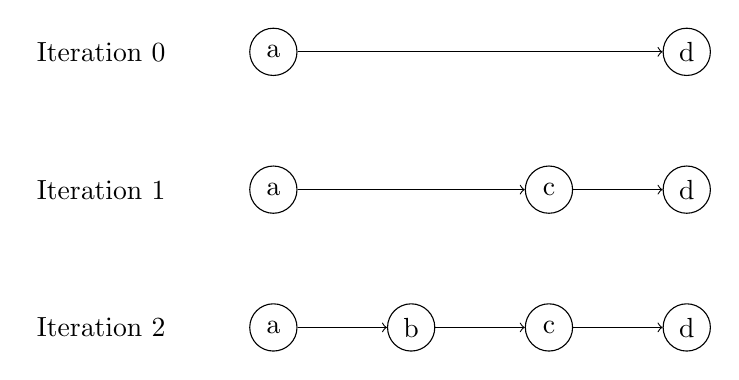
\begin{tikzpicture}
        \node[align=left] at (1.75*-1.25,1.75*2) {Iteration 0};
        \node[circle, draw, minimum size=0.6cm, inner sep=0pt] at (1.75*0.0, 1.75*2.0)  (a_0)    {a};
        \node[circle, draw, minimum size=0.6cm, inner sep=0pt] at (1.75*3.0, 1.75*2.0)  (d_0)    {d};
        \draw[->]  (a_0) edge node {} (d_0);

        \node[align=left] at (1.75*-1.25,1.75*1) {Iteration 1};
        \node[circle, draw, minimum size=0.6cm, inner sep=0pt] at (1.75*0.0, 1.75*1.0)  (a_1)    {a};
        \node[circle, draw, minimum size=0.6cm, inner sep=0pt] at (1.75*2.0, 1.75*1.0)  (c_1)    {c};
        \node[circle, draw, minimum size=0.6cm, inner sep=0pt] at (1.75*3.0, 1.75*1.0)  (d_1)    {d};
        \draw[->]  (a_1) edge node {} (c_1);
        \draw[->]  (c_1) edge node {} (d_1);

        \node[align=left] at (1.75*-1.25,1.75*0) {Iteration 2};
        \node[circle, draw, minimum size=0.6cm, inner sep=0pt] at (1.75*0.0, 1.75*0.0)  (a_2)    {a};
        \node[circle, draw, minimum size=0.6cm, inner sep=0pt] at (1.75*1.0, 1.75*0.0)  (b_2)    {b};
        \node[circle, draw, minimum size=0.6cm, inner sep=0pt] at (1.75*2.0, 1.75*0.0)  (c_2)    {c};
        \node[circle, draw, minimum size=0.6cm, inner sep=0pt] at (1.75*3.0, 1.75*0.0)  (d_2)    {d};
        \draw[->]  (a_2) edge node {} (b_2);
        \draw[->]  (b_2) edge node {} (c_2);
        \draw[->]  (c_2) edge node {} (d_2);
    \end{tikzpicture}
    \caption{Beispiel des iterativen Ersetzen von Abkürzungen}
\end{figure}

Um diese Funktion zu erhalten, müssen die Abkürzungen, welche beim Kontraktieren des Graphens eingefügt werden, mitsamt dem übersprungenen Knoten gesammelt werden.
Das Algorithmus betrachtet den Pfad mit Abkürzungen als Stapel und bearbeitet jeweils nur die beiden obersten Knoten, da das Einfügen in ein Array an einer bestimmte Stelle für einen Computer Rechenintensiver ist.

\begin{algorithm}[ht]
    \caption{Shortcut replacement}
    \begin{algorithmic}[1]
        \Require Pfad $p$ mit Abkürzungen, Abkürzungungsfunktion $S \colon V \times V \to V \cup \{ {none} \}$
        \Ensure Pfad $p'$ ohne Shortcuts

        \If {$\text{len}(p) == 1$}
        \State \Return $p$
        \EndIf
        \State

        \State $p' \leftarrow ()$
        \State

        \While {$\text{len}(p) >= 2$}
        \State $w \leftarrow \text{pop}(p)$
        \State $u \leftarrow \text{pop}(p)$
        \State $v \leftarrow S((u, w))$
        \State

        \If {$v \neq none$}
        \State $\text{push}(p, u)$
        \State $\text{push}(p, v)$
        \State $\text{push}(p, w)$
        \Else
        \State $\text{push}(p, u)$
        \State $\text{push}(p', w)$
        \EndIf
        \EndWhile

        \State
        \State $p' \leftarrow \text{reversed}(p')$

        \State
        \State \Return $p'$
    \end{algorithmic}
    \label{ch:alg:shortcut_replacement}
\end{algorithm}

\subsection{Early stop}

Der Algorithmus \ref{ch:query_simple} ist von theoretischer Bedeutung.
Implementierungen ähneln einer bidirektionalen Dijkstra Suche, es werden also abwechselnd Knoten der Upward Suche und der Downard Suche expandiert.
Die Expansion einer Suchrrichtung kann dabei gestopt werden, wenn die kleinste Distanz der Vorwärtswarteschlange größer als die bisherige kleinge Treffpunkt-Distanz.

\subsection{Stall-on-demand}

Wie \autoref{graphs:fig:counterexample_uptimal_upward} zeigt, die im Upward und Downward Graphen gefunden Distanzen nicht optimal sein.
Für das finden einen küzesten Pfades sind jedoch nur die Knoten interesannt, deren Distanz optimal ist.
Mit der von \cite{schultes2007dynamic} vorgestellten Methode \emph{stall-on-demand} ist es möglich, den Suchraum der beiden Teilsuchen zu verkleinern.
Hiefür wird die Expansion eines Knotens abgebrochen, wenn er durch eine Kante des jeweils anderen Graphen günstiger erreicht werden kann.

\begin{definition}[stall-on-demand]
    Sei $C = (G_u, G_d)$ ein Contracted Graph mit $G_u = (V, E_u)$ und $G_d = (V, E_d)$.
    Der Knoten $u \in V$ hat keine optimale Distanz in der Dijkstra suche von $s$ in $G_u$, wenn zum Zeitpunkt seiner Expansion es eine Kante $(u, v, d) \in E_d$, $v \in V$, $d \in \mathbb{R}$ gibt mit ${dist}(v) + d < {dist}(u)$.
    Die Expansion von $u$ kann dann abgebrochen werden, die aus $u$ ausgehenden Kanten müssen nicht betrachtet werden.
    Gleiches gilt analog für $G_d$.
\end{definition}

Betrachten wird dies an dem Beispiel in \autoref{fig:ch:stall_example}.
Die blauen Kanten sind dabei Kanten der Upward Suche, die rote Kante eine von $u$ ausgehende Downward Kante.
Bisher wurde $v$ mit einer Distanz von eins expandiert, als nächstes soll $u$ expandiert werden.
$u$ hat die Distanz drei in der Upward Suche, kann durch die Verwendung der Upward Kante mit der Distanz zwei erreicht werden, also ist die Distanz drei nicht optimal und von $u$ ausgehenden Kanten müssen nicht relaxiert werden.

\begin{figure}
    \centering
    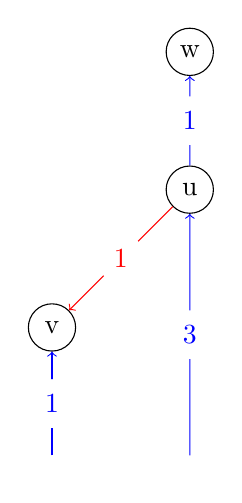
\begin{tikzpicture}[scale=1.75]
        \node[circle, draw, minimum size=0.6cm, inner sep=0pt] at (0, 1)  (v)    {v};
        \node[circle, draw, minimum size=0.6cm, inner sep=0pt] at (1, 2)  (u)    {u};
        \node[circle, draw, minimum size=0.6cm, inner sep=0pt] at (1, 3)  (w)    {w};

        \node[] at (0, 0)  (uv)    {};
        \node[] at (1, 0)  (uu)    {};

        \draw[->,blue]  (u) edge node[circle, fill=white] {1} (w);

        \draw[->,red]  (u) edge node[circle, fill=white] {1} (v);

        \draw[->,blue]  (uv) edge node[circle, fill=white] {1} (v);
        \draw[->,blue]  (uu) edge node[circle, fill=white] {3} (u);
    \end{tikzpicture}
    \caption{Beispiel stall-on-demand}
    \label{fig:ch:stall_example}
\end{figure}

\subsection{Erstellung}

Ein Contracted Graph wird durch die vollständige Kontraktion eines Graphens erstellt, wobei die Reihenfolge, in der die Knoten kontraktiert werden entweder im Vorraus fest steht oder während der Kontraktion des Graphens erstellt, indem der jeweils \emph{unwichtigste} Knoten zuerste kontraktiert wird.

\paragraph{Top-Down}

Bei der Top-Down Kontraktion ist die level-to-vertex Funktion ${ltv}$ vorgegeben.
Die Knoten werden in Reihenfolge ihres Levels kontrakiert, wobei mit dem niedrigsten Level begonnen wird.
Hierbei sind beliebige Sortierungen denkbar, die Auswahl ist nicht vollständig.

\todo{Funke fragen. Was für Sortierungen soll ich vorstellen?}

Die Knoten werden zufällig auf die Level verteilt.


\subparagraph{Sortiert nach Grad}
Die Knoten werden nach ihrem Grad sortiert, wobei die kleinsten Grade zuerst kontraktiert werden.
Die überlegung dahinter ist, dass Knoten mit vielen Nachbarn auch viele neue Kanten einfügen können, was vermieden werden soll.
Nach größtem Grad ist vielleicht auch spannend.


\paragraph{Bottom-Up}

Bei der Bottom-Up contraction wird die vertex-to-level Funktion ${vtl}$ währen der Kontraktion erstellt.
Dafür wird mit einer Heuristik der jeweils nächst \emph{unwichtigste} Knoten ausgewählt, kontraktiert und dem nächstem Level zugewiesen.
Ein unwichtiger Knoten hat hierbei einen niedrigen Heuristik-Wert.
Die in der Praxis am meist-verwendeten Heurisiken beinhalten die \emph{Kanten-Differenz}.
Sie gibt an wie sich die Anzahl der Kanten im gesammten Graph durch die Kontraktion verändert.
Sie wird durch die Anzahl der neu hinzugefügten Kanten subtrahiert durch die Anzahl der entfernten Kanten gebildet.
Die Kontraktion eines Knoten kann dabei die Heurisitk-Werte anderer Knoten verändern.
Damit jedes mal der Knoten mit der niedrigsten Heuristik ausgewählt wird, müssen nach jeder Kontraktion alle Heuristik-Werte neuberechnet werden.
Dies ist im Allgemeinen jedoch zu teuer ist, weshalb in der Praxis sich zwei Methoden als effektiv gezeigt haben:

Beim \emph{Lazy poping} besteht die Annahme, dass ein Knoten nur wichtiger werden kann.
Aus der Warteschlange wird ein Knoten entnommen und geprüft, ob sein Heuristik-Wert noch gleich ist.
Wenn er noch gleich ist, wird er kontraktiert, wenn nicht wird er zurück die Warteschlange gepusht.
Dies wird wiederholt, bis schließlich ein Knoten gefunden wird.

Beim \emph{Neighbor update} werden nach der Kontraktion eines Knoten die Heuristik Werte der Nachbarn geupdated.
Es lässt sich zeigen, dass sich die Kanten-Differenz von Nachbarn zweiter Ordnung nur in Ausnahmfällen ändert.\todo{Oder?}

Um die zu einem Contracted Graph dazugehörige Shortcut-Funktion zu erhalten, muss während der Kontraktion des Graphens eine Liste der Shortcuts erstellt werden.
Wird die im vorherigen Absatz erwähnte abgeschwächte Befingung verwenden, muss darauf geachtet werden, dass sich der kürzeste Shortcut zweier Knoten während der Kontraktion des Graphens mehrmals ändern kann.
Für die Shortcut-Funktion darf nur der als letzte gesetzte, beste Shortcut verwendet werden.

\section{Hierachical Hub Labeling}\label{chapter:hl}

Die Contracted Graph Anfrage ohne Stopbedingung erstellt jeweils den vollen Suchbaum für den Start und Zielknoten und sucht aus den expaniderten Knoten den Knoten mit geringester Summe der Distanzen in beiden Suchen.
Die Idee des Label ist es, den Suchbaum des upward bzw. downard Graphenz zu speichern, eine $s-t$-Anfrage ist dann nur noch der vergleich zweier Label.
Ein kürzester Pfad wird gefunden, in dem der Knoten mit der geringsten Summe der Distanzen des forwad und backward Labels gefunden wird.
In der in \cite{abraham2011hub} vorgestellten Terminioligy wird das Label des upward Graphen \emph{forward Label} und das des Downward Graphen \emph{backward Label} genannt.

\begin{definition}[Hub Graph]
    Sei $G = (V, E)$. $H = (L_f, L_b)$ ist ein \emph{Hub Graph} und es gilt:
    Die Forward-Label Funktion $L_f \colon V \to V \times \mathbb{R}^+_0$ weist jedem Knoten ein Forward Label zu.
    Sei $L_f (u)$ das Forward Label des Knotens $u \in V$, dann gibt es für jeden Knoten $v \in V$ höchstens ein $(v, d) \in L_f (u)$ und es gilt $d \geq {spd}_G((u, v))$.
    Ein Backward Label ist ein Forward Label des Umkehrgraphens $G^T$.

    Zusammen erfüllen die Forward Label und die Backward Label die Abdeckungseigenschaft:
    Für jedes Knotenpaar $s, t \in V$ für die es einen kürzesten $s-t$ Pfad gibt, gibt es einen Knoten $m \in V$ mit $(m, d_f) \in L_f (s)$, $(m, d_r) \in L_r$ und $d_f + d_r = {spd}_G ((s, t))$.
\end{definition}

Die Definition der Label ähnelt bereits dem Beweis der Korrektheit der Contracted Graph Query, bei diesem wurde ebenfalls mit dem Treffpunktknoten $m$ argumentiert.
Aus einem Contracted Graphen lässt sich ein Hub Graph bauen, indem der Suchbaum des Upward Graphen als Forward Label und der des Downward Graphen als Backward LAbel betrachtet wird, denn die Suchbäume treffen sich im Knote mit dem Höchstem Level mit optimalem Abstand.
Die Erstellung kann auf zwei Wegen geschehen, durch eine Dijkstra Suche im Upward bzw. Downward Graphen pro Knoten oder durch \emph{Merging}.
Diese so erstelten Labels sind hierarisch: Es gibt eine Ordnung der Knoten (die vertex-to-level Funktion), so dass das Forward und das Backward Label eines Knotens $u$ nur Knoten $h$ mit höherer Ordnung enthält.
Es sind auch Label möglich, die diese Eigenschaft nicht erfüllen, weiter könnnen solche für manche Graphen deutlich kleiner sein, als hierarische.\cite{goldberg2013separating}

\subsubsection{Query}

Sei $H = (L_f, L_b)$ ein Hub Graph.
Algorithmus \ref{hl:alg:query} zeigt wie wenig Schritte dafür notwendig sind, eine kürzeste Pfad Distanz in $H$ zu finden, nur noch das Finden des Knotens mit der geringsten Summe der Distanzen ist dafür notwendig.
Der Brweis der Korrektheit


\begin{algorithm}[ht]
    \caption{Hub Label Query}
    \begin{algorithmic}[1]
        \Require Forward Label Funktion $L_f$, Backward Label Funktion $L_b$, Startknoten $s \in V$, Zielknoten $t \in V$
        \Ensure Treffknoten $m \in V \cup \{ {none} \}$, ${dist}_u$
        \State $l_s \leftarrow L_f (s)$
        \State $l_t \leftarrow L_b (t)$

        \State
        \State $m \leftarrow {none}$
        \State $d \leftarrow \infty$

        \ForAll {$v \in V \colon (v, d_f) \in l_s \land (v, d_r) \in l_t$}
        \If {$d_f + d_r < d$}
        \State $d \leftarrow d_f + d_r$
        \State $m \leftarrow v$
        \EndIf
        \EndFor

        \State
        \State \Return $m$, $d$
    \end{algorithmic}
    \label{hl:alg:query}
\end{algorithm}

\subsection{Pfad erstellung}

Um nachdem ein Treffpunkt-Knoten $m$ gefunden wurde einen Pfad erstellen zu können sind noch zusätzliche Information notwendig, damit im ersten Schritt der Pfad in den Suchbäumen erstellt werden kann und im zweiten Schritt die Abkürzungen ersetzt werden können.
Um den Pfad im Suchbaum zu zu erstellen, muss für jeden Knoten in dem Label sein Vorgänger, falls vorhanden, bekannt sein.
Dafür wird die Label Definition von einer Teilmenge von $V \times \mathbb{R}$ erweitert auf eine Teilmenge von $V \times \mathbb{R} \times V \cup \{ none \} $, der zusätzliche Knoten speichert hierbei den Vorgängern.
Für das erstellen eines Pfades springt man, beginnend vom Treffpunkt-Knoten durch alle Vorgänger, bis es keinen Vorgänger mehr gibt.
Durch das ersetzen der Abkürzungen, etwa mit dem Algorithmus \ref{ch:alg:shortcut_replacement}, erhält man so einen gültigen PFad auf $G$.

\subsection{Datenstruktur}

Gibt es Totalordnung der Knoten, dann lässtsich durche eine geschickte Wahl der Datenstruktur zur Speicherung eines LAbels der Knoten mit der geringsten Summe der Distanzen in linearer Zeit zur Größe der Label finden:
Label sind dann eine Liste und Elemente der Label sind nach dem Knoten sortiert.
Ähnlich wie bei Merge Sort werden dabei die Einträge Pärchenweise verglichen, wobei der Index des LAbels mit dem jeweils kleineren Element incrementiert wird.
Dadurch ist garantiert, dass alle Knoten, welche in beiden Labeln vorhanden sind, Zeitgleich betrachtet werden und falls diese einen aktuell besten Treffpunkt-Knoten bilden, diese INformation gespeichert werden kann.

Um das Finden der Vorgänger effizienter zu machen, wird nicht der Vorgänger selbst gespeichert, sondern sein Index im Label.
\autoref{ch:fig:label} zeigt ein Label solcher Art.

\begin{figure}[ht]
    \centering
    \begin{tabular}{@{}llllll@{}}
        \toprule
        Index           &  & 0   & 1   & 2   & 2 \\ \midrule
        Vertex          &  & $e$ & $j$ & $k$ &   \\
        Distanz         &  & 0   & 3   & 2   &   \\
        Vorgänger Index &  & -   & 2   & 0   &   \\ \bottomrule
    \end{tabular}
    \caption{Beispiel eines Labels}
    \label{ch:fig:label}
\end{figure}

\subsection{Erstellung}

Da die LAbel den expandierten Knoten im Suchbaum des Upward bzw. Downard Graph enstpricht, können diese naive dadurch gebildet werden, dass pro Knoten der enstprechende Suchbaum mit einer Dijkstra Suche erstellt wird und die gefundenen Knoten ensprechend sortiert werden.
Dies lässt sich gut parallelisieren, ist jedocht gibt es eine Methode, welche meist effizienter ist

\subsubsection{Merging}

Für jeden Knoten des Graphens $G$ wird ein Label erstellt, das zu beginnt nur den Knoten selbst enthält.
Danach werden die Label in der Reihenfolge der Level, von groß zu klein, wie folgt erstellt:
Pro Knoten werden die ausgehenden Kanten des Downard bzw. Upward Graphens betrachtet.
Die Köpfe dieser Kanten haben ein höheres Level als der Knoten selbst, daher exisiterien ihren Label bereits.
Sie werden gemerged, indem sie zusammen ein neues LAbel bilden und Duplikate mit größerer Distanz entfernt werden.
Dies erstellt ebenfalls die benötigten

\subsubsection{Pruning}

Die erstellten Label enthalten bisher noch Knoten mit nicht-optimaler Distanz in $G$ (siehe \autoref{graphs:fig:counterexample_uptimal_upward}), was einerseits den Speicherbedarf der  Label als auch die Abfrage Zeiten erhöht.
Die Einträge mit nicht-optimaler Distanz können dabei entfernt werden, indem die erstellten Hub Label selbst dafür benutzt werden, die Einträge mit nicht-optimaler Distanz zu identifizieren.
Beim Merging kann dies auch bereits während der ERstelltung geschehen, da die Labels von Knoten mit höherem Level beretis existieren.